%%%%%%%%%%%%%%%%%%%%%%%%%%%%%%%%%%%%%%%%%%%%%%%%%%%%%%%%
\documentclass[12pt,a4paper]{article}% 文档格式
\usepackage{ctex,hyperref}% 输出汉字
\usepackage{times}% 英文使用Times New Roman
%%%%%%%%%%%%%%%%%%%%%%%%%%%%%%%%%%%%%%%%%%%%%%%%%%%%%%%%
\title{\fontsize{18pt}{27pt}\selectfont% 小四字号,1.5倍行距
	{\heiti% 黑体 
	CaO结构的第一性原理研究}}% 题目
%%%%%%%%%%%%%%%%%%%%%%%%%%%%%%%%%%%%%%%%%%%%%%%%%%%%%%%%
\author{\fontsize{12pt}{18pt}\selectfont% 小四字号,1.5倍行距
	{\fangsong% 仿宋
		邱子杰~黄佳炜}\\% 标题栏脚注
	\fontsize{10.5pt}{15.75pt}\selectfont% 五号字号,1.5倍行距
	{\fangsong% 仿宋
		(福州大学~~~物理与信息工程学院、微电子学院)}}% 作者单位,“~”表示空格
%%%%%%%%%%%%%%%%%%%%%%%%%%%%%%%%%%%%%%%%%%%%%%%%%%%%%%%%
\date{}% 日期(这里避免生成日期)
%%%%%%%%%%%%%%%%%%%%%%%%%%%%%%%%%%%%%%%%%%%%%%%%%%%%%%%%
\usepackage{amsmath,amsfonts,amssymb}% 为公式输入创造条件的宏包
%%%%%%%%%%%%%%%%%%%%%%%%%%%%%%%%%%%%%%%%%%%%%%%%%%%%%%%%
\usepackage{graphicx}% 图片插入宏包
\usepackage{subfigure}% 并排子图
\usepackage{float}% 浮动环境,用于调整图片位置
\usepackage[export]{adjustbox}% 防止过宽的图片
%%%%%%%%%%%%%%%%%%%%%%%%%%%%%%%%%%%%%%%%%%%%%%%%%%%%%%%%
\usepackage{bibentry}
\usepackage{natbib}% 以上2个为参考文献宏包
%%%%%%%%%%%%%%%%%%%%%%%%%%%%%%%%%%%%%%%%%%%%%%%%%%%%%%%%
\usepackage{abstract}% 两栏文档,一栏摘要及关键字宏包
\renewcommand{\abstracttextfont}{\fangsong}% 摘要内容字体为仿宋
\renewcommand{\abstractname}{\textbf{摘\quad 要}}% 更改摘要二字的样式
%%%%%%%%%%%%%%%%%%%%%%%%%%%%%%%%%%%%%%%%%%%%%%%%%%%%%%%%
\usepackage{xcolor}% 字体颜色宏包
\newcommand{\red}[1]{\textcolor[rgb]{1.00,0.00,0.00}{#1}}
\newcommand{\blue}[1]{\textcolor[rgb]{0.00,0.00,1.00}{#1}}
\newcommand{\green}[1]{\textcolor[rgb]{0.00,1.00,0.00}{#1}}
\newcommand{\darkblue}[1]
{\textcolor[rgb]{0.00,0.00,0.50}{#1}}
\newcommand{\darkgreen}[1]
{\textcolor[rgb]{0.00,0.37,0.00}{#1}}
\newcommand{\darkred}[1]{\textcolor[rgb]{0.60,0.00,0.00}{#1}}
\newcommand{\brown}[1]{\textcolor[rgb]{0.50,0.30,0.00}{#1}}
\newcommand{\purple}[1]{\textcolor[rgb]{0.50,0.00,0.50}{#1}}% 为使用方便而编辑的新指令
%%%%%%%%%%%%%%%%%%%%%%%%%%%%%%%%%%%%%%%%%%%%%%%%%%%%%%%%
\usepackage{url}% 超链接
\usepackage{bm}% 加粗部分公式
\usepackage{multirow}
\usepackage{booktabs}
\usepackage{epstopdf}
\usepackage{epsfig}
\usepackage{longtable}% 长表格
\usepackage{supertabular}% 跨页表格
\usepackage{algorithm}
\usepackage{algorithmic}
\usepackage{tabu}
\usepackage{threeparttable}
\usepackage{changepage}% 换页
\newcommand{\upcite}[1]{\textsuperscript{\textsuperscript{\cite{#1}}}}
%%%%%%%%%%%%%%%%%%%%%%%%%%%%%%%%%%%%%%%%%%%%%%%%%%%%%%%%
\usepackage{enumerate}% 短编号
\usepackage{caption}% 设置标题
\captionsetup[figure]{name=\fontsize{10pt}{15pt}\selectfont Figure}% 设置图片编号头
\captionsetup[table]{name=\fontsize{10pt}{15pt}\selectfont Table}% 设置表格编号头
%%%%%%%%%%%%%%%%%%%%%%%%%%%%%%%%%%%%%%%%%%%%%%%%%%%%%%%%
\usepackage{indentfirst}% 中文首行缩进
\usepackage[left=2.50cm,right=2.50cm,top=2.80cm,bottom=2.50cm]{geometry}% 页边距设置
\renewcommand{\baselinestretch}{1.5}% 定义行间距(1.5)
%%%%%%%%%%%%%%%%%%%%%%%%%%%%%%%%%%%%%%%%%%%%%%%%%%%%%%%%
\usepackage{fancyhdr} %设置全文页眉、页脚的格式
\pagestyle{fancy}
\hypersetup{colorlinks=true,linkcolor=black}% 去除引用红框,改变颜色
%%%%%%%%%%%%%%%%%%%%%%%%%%%%%%%%%%%%%%%%%%%%%%%%%%%%%%%%
\begin{document}% 以下为正文内容
	\maketitle% 产生标题,没有它无法显示标题
	%%%%%%%%%%%%%%%%%%%%%%%%%%%%%%%%%%%%%%%%%%%%%%%%%%%%%%%%
	\lhead{}% 页眉左边设为空
	\chead{}% 页眉中间设为空
	\rhead{}% 页眉右边设为空
	\lfoot{}% 页脚左边设为空
	\cfoot{\thepage}% 页脚中间显示页码
	\rfoot{}% 页脚右边设为空
	%%%%%%%%%%%%%%%%%%%%%%%%%%%%%%%%%%%%%%%%%%%%%%%%%%%%%%%%
	\begin{abstract}
		\fangsong 基于氧化钙在各个领域有广泛的应用,需求量不断增大,本文对氧化钙的能带结构,态密度及电子结构进行了系统的研究。采用基于密度泛函理论的第一性原理平面波赝势理
		论方法对晶体进行了理论计算与分析.优化后所得晶格常数与实验值基本一致.研究结果表明 CaO 晶体属于直接带隙绝缘体,带隙值为 4.578 eV,Ca 与 O 之间的电子云重叠比 Ca 与 Ca 之间的强,使得 Ca—O 共价键强
		于 Ca—Ca 键。
	\end{abstract}
	
	\begin{adjustwidth}{1.06cm}{1.06cm}
		\fontsize{10.5pt}{15.75pt}\selectfont{\heiti{关键词:}\fangsong{CaO、电子结构、第一性原理、晶体结构}}\\
	\end{adjustwidth}
	\section{引言}
	金属氧化物是一类在催化作用、微电子和光电设
	备等领域应用广泛的材料$^{[1-4]}$,其中碱土金属氧化物是地球地下幔的重要成分,是一种广泛应用的工业科学技术基础材料$^{[5-6]}$。氧化钙(CaO)便是其中的一种。氧化钙俗称生石灰,微溶于水不溶于醇,可溶于酸、甘油等溶剂。主要应用于水泥、
	玻璃、陶瓷行业,也经常作为制药、非铁金属、肥
	料、皮革等多种领域的无机填料口,在实验室中经常
	用于氨气的干燥、醇类脱水、制备过氧化钙等,因此氧
	化钙一直受到广泛的研究关注。近年来,CaO的用途不断发展,应用
	领域不断扩大,需求量逐渐增加.因此,不同条件下
	CaO晶体的电子结构和光学性质有待进一步研究.目
	前,通过掺杂改变CaO带隙和光电性质的研究已有
	报道。大量实验和理论研究证明,施加压强和掺杂
	都能够有效改变材料的带隙和光电性质,而通过施加
	压强调控CaO光电性质的报道却少有涉及$^{[7-9]}$。本研究
	通过密度泛函理论对CaO的能带结构、态密度进行计算分析,以期为后续实
	验研究提供一定的理论依据。
	\section{模型构建和计算方法}
	\subsection{模型构建}
	本研究选用的模型是CaO晶体,为离子晶体结
	构,属于FM-3M空间群,几何优化后晶格常数为a=b=c=0.4810 \textbf{nm}。
	本研究选用CaO原胞作为研究对象,其结构如图1
	所示.由图l可以看出,CaO原胞中共有2种原子。l中绿色球代表Ca原子,红
	色球代表O原子.
	\begin{figure}[H]
		\centering
		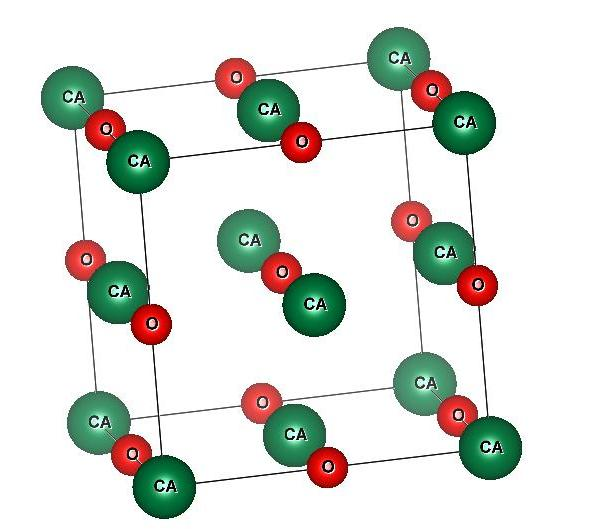
\includegraphics[width=0.45\linewidth]{img/CaO}
		\caption[Cao的晶胞结构图]{CaO的晶胞结构图}
		\label{fig:cao}
	\end{figure}
	\subsection{计算方法}
	基于第一性原理,利用 Materials Studio 软件包中的 CASTEP(cambridge sequential total energy package) 完成计算.采用基于平面波基组的超软赝势(ultrasoft pseudo potential)描述离子实和价电子之间的相互作用势,选取 O(2s$^2$2p$^4$)和 Ca(3s$^2$3p$^6$4s$^2$)组态电子作为价电子,其他轨道电子作为离子实,电子波函数采用平
	面波基组展开.交换关联能选用广义 梯度近似(generalized gradient approximation, GGA)处理,为保证计算的精确性,优化收敛的容许条件设为:原子间的相互作用
	小于0.1 eV/μm,分应力小于0.02 GPa,自洽计算的公差容许值为 5.0 eV/atom. 原胞中的价电子波函数用平面波基矢展开并设平面波的截断能为400 eV,迭代收敛准确度为 $10^{-4}$ eV,选取广义梯度近似处理交	
	换关联能部分,交换关联势计算采用(PerdewBurker
	Ernzerhof,PBE)提出 GGA,采用超软贋势
	计算总能量在倒易空间中进行,布里渊区积分采用$4\times4\times4$的  Monkhorst-Pack 方法.
	\section{结果与讨论}
	\subsection{体系优化}
	为了得到体系的稳定结构,在CaO实验晶格
	常数值$^{[10]}$附近对原胞体积和总能量进行了优化计算。
	通过计算这些不同原胞体积下体系的总能量.得出了CaO的晶格常数a、b、c.表1是CaO正交相结构优化后的晶格常数.
	\begin{table}[H]
		\begin{center}
			\caption{CaO正交结构优化后的晶格常数}
			\resizebox{\textwidth}{!}
			{\begin{tabular}{c c c c }
					\toprule[2pt]
					\multicolumn{1}{m{3cm}}{\centering \textbf{物理参量}}	&\multicolumn{1}{m{3cm}}{\centering \textbf{实验值} }&\multicolumn{1}{m{3cm}}{\centering \textbf{理论值} }&\multicolumn{1}{m{3cm}}{\centering \textbf{误差}$\%$ }\\
					\midrule
					a/nm & 0.4834 &0.4810 &0.49$\%$\\
					b/nm & 0.4834 &0.4810 & 0.49$\%$  \\
					c/nm & 0.4834 &0.4810 & 0.49$\%$ \\
					\bottomrule[2pt]
			\end{tabular}}
		\end{center}
	\end{table}
	\vspace{-0.8cm}
	由表1可看出,几何优化
	后得到的理论晶胞参数与实验值非常接近.这也保证了计算结果的可靠性。
	\subsection{电子结构}
	从图2(a)可以看到CaO的总态密度具有约4.578 eV的带隙。费米能级以下部分是价带,而费米
	能级以上部分则为导带。其中这些价带被分为多个成键峰,这些成键峰主要由Ca-p,Ca-d和O-p,O-s轨道杂化来形成。从CaO总态密度和各原子分态密度图中,我们还可以看出,CaO的
	价带分为下述个部分:-20 $\sim$-14.85 eV处的峰值主要由O的s态贡献,同时Ca的p态也有少量贡献。带价顶部主要由Ca的d态贡献,并参杂O的p态。带价底部的态密度主要由O的p态贡献,并掺杂Ca的d态。
	\begin{figure}[H]
		\centering    
		\subfigure[CaO的总态密度图]{				% 图片1([]内为子图标题)						
			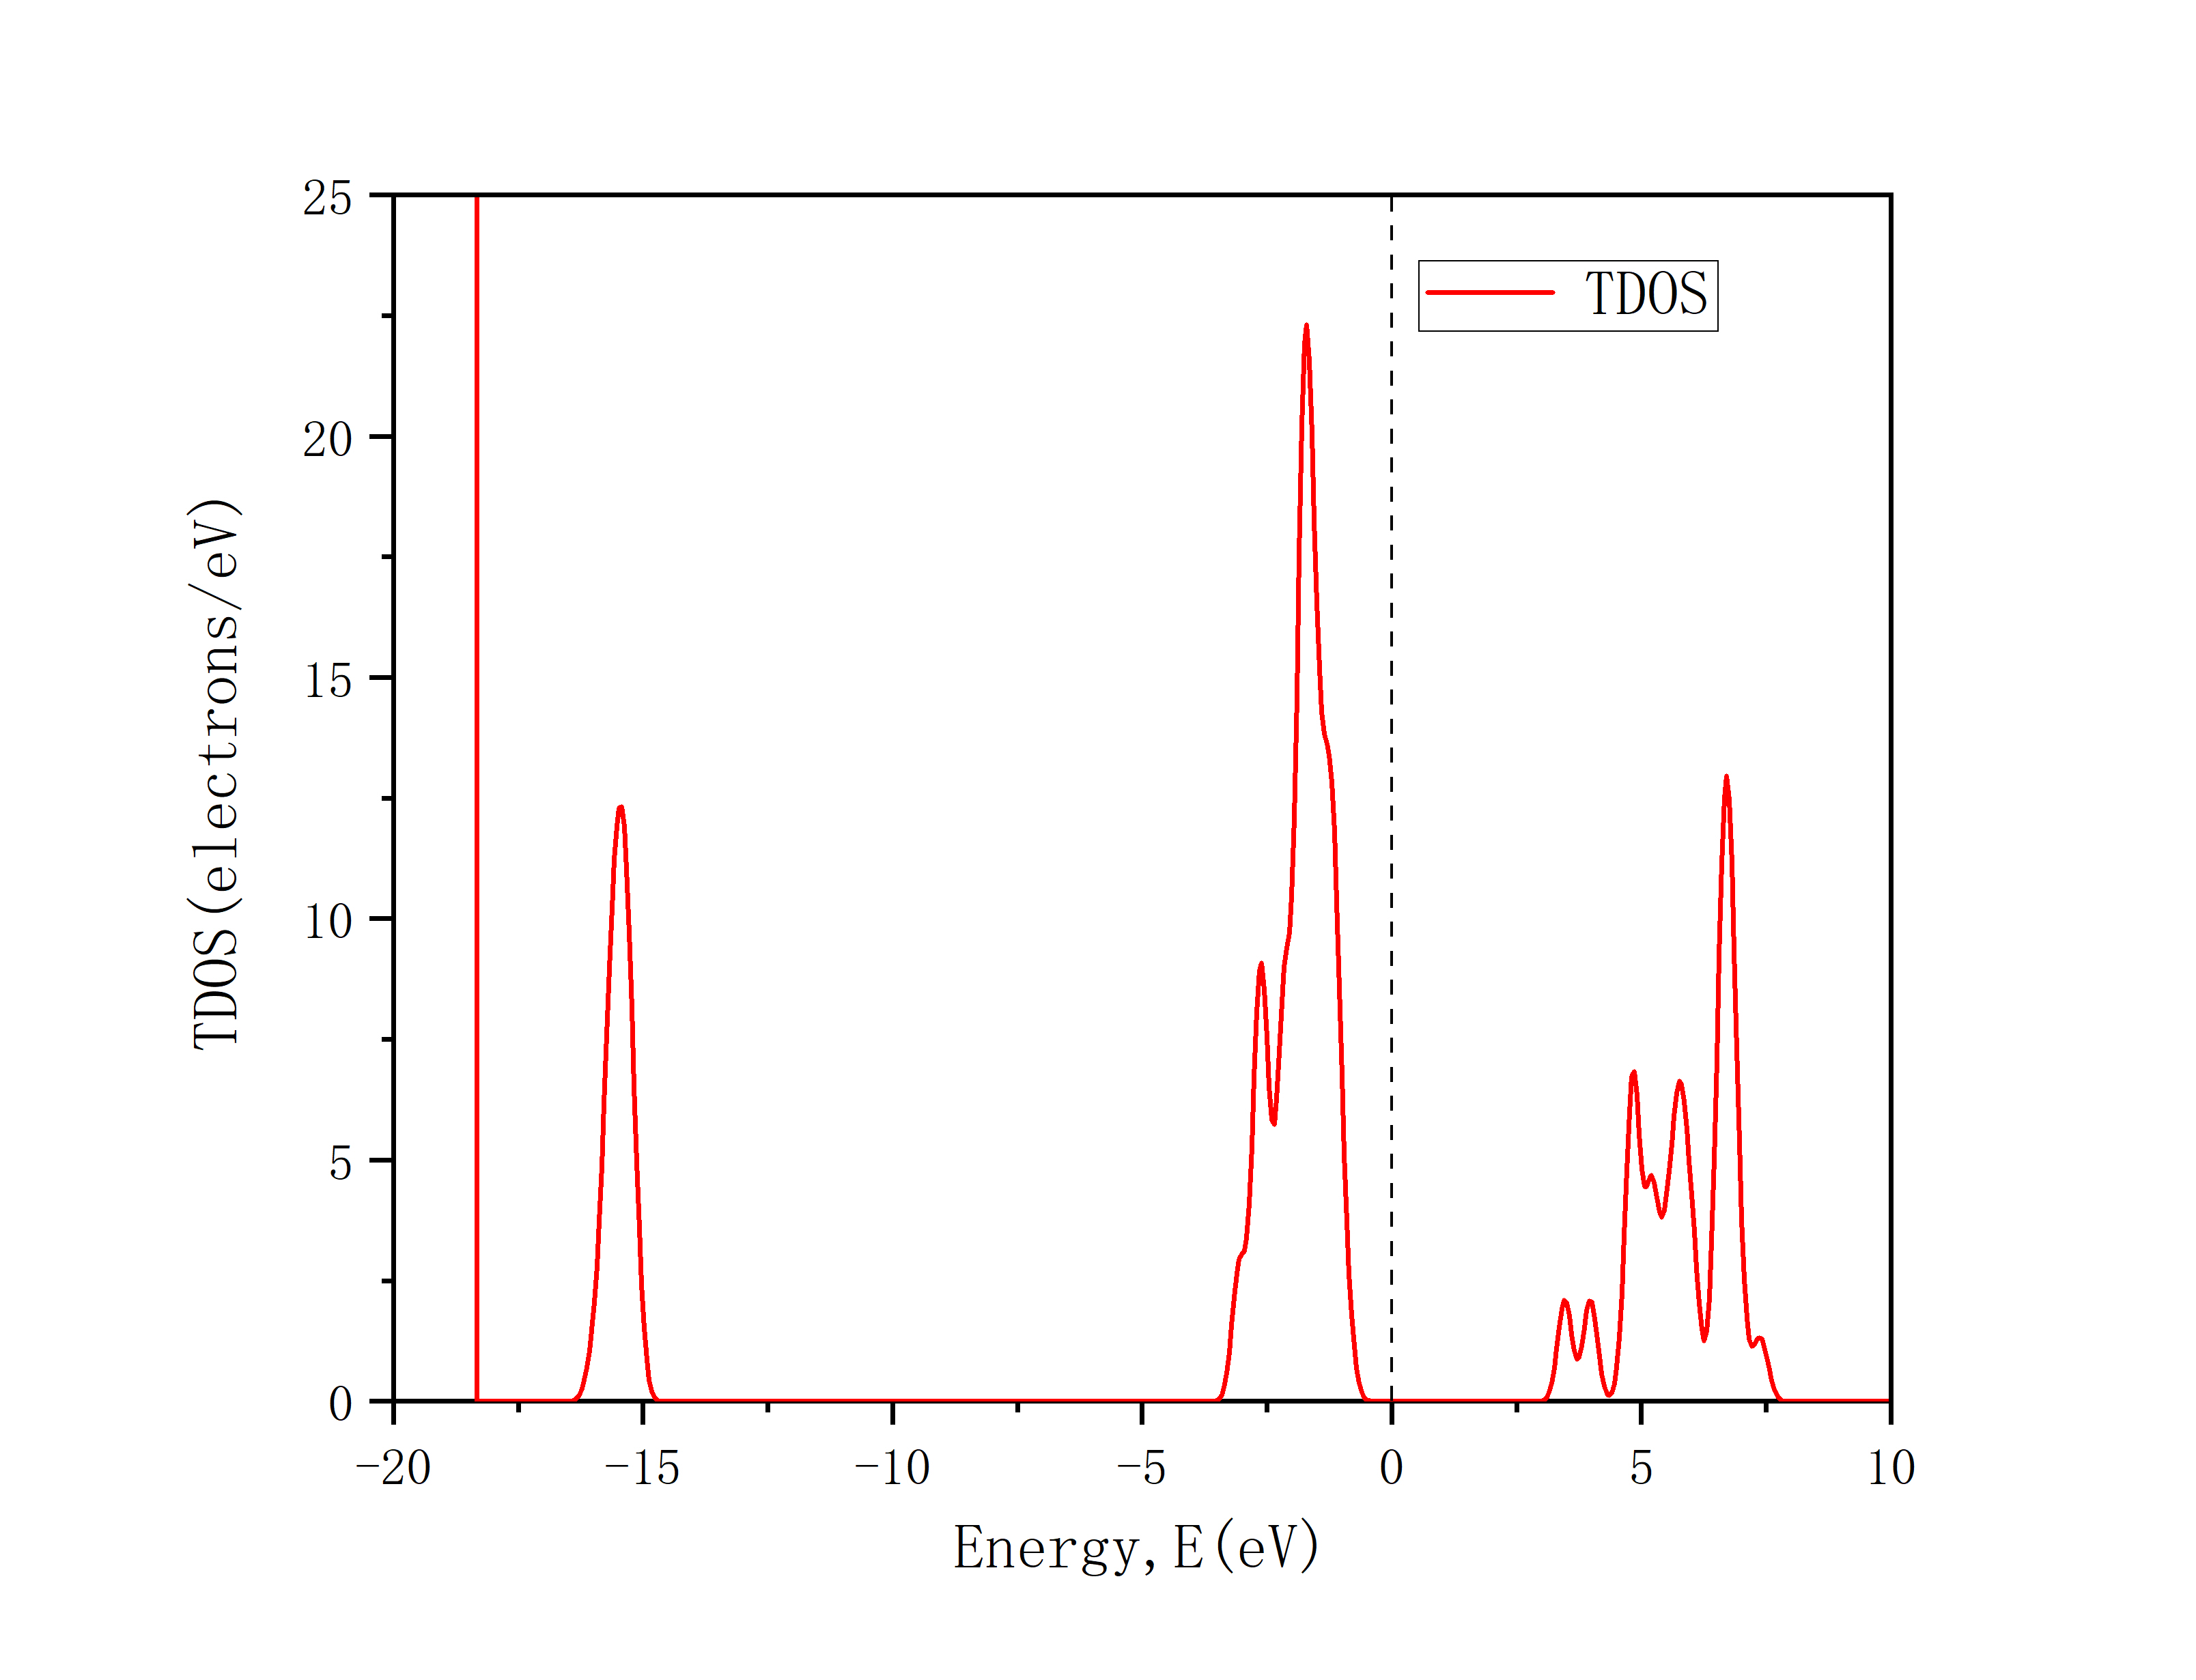
\includegraphics[width=0.43\textwidth]{img/TDOS (1).jpg}}			  % 子图1的图片宽度 不能空行
		\subfigure[Ca的分波态密度图]{				% 图片2
			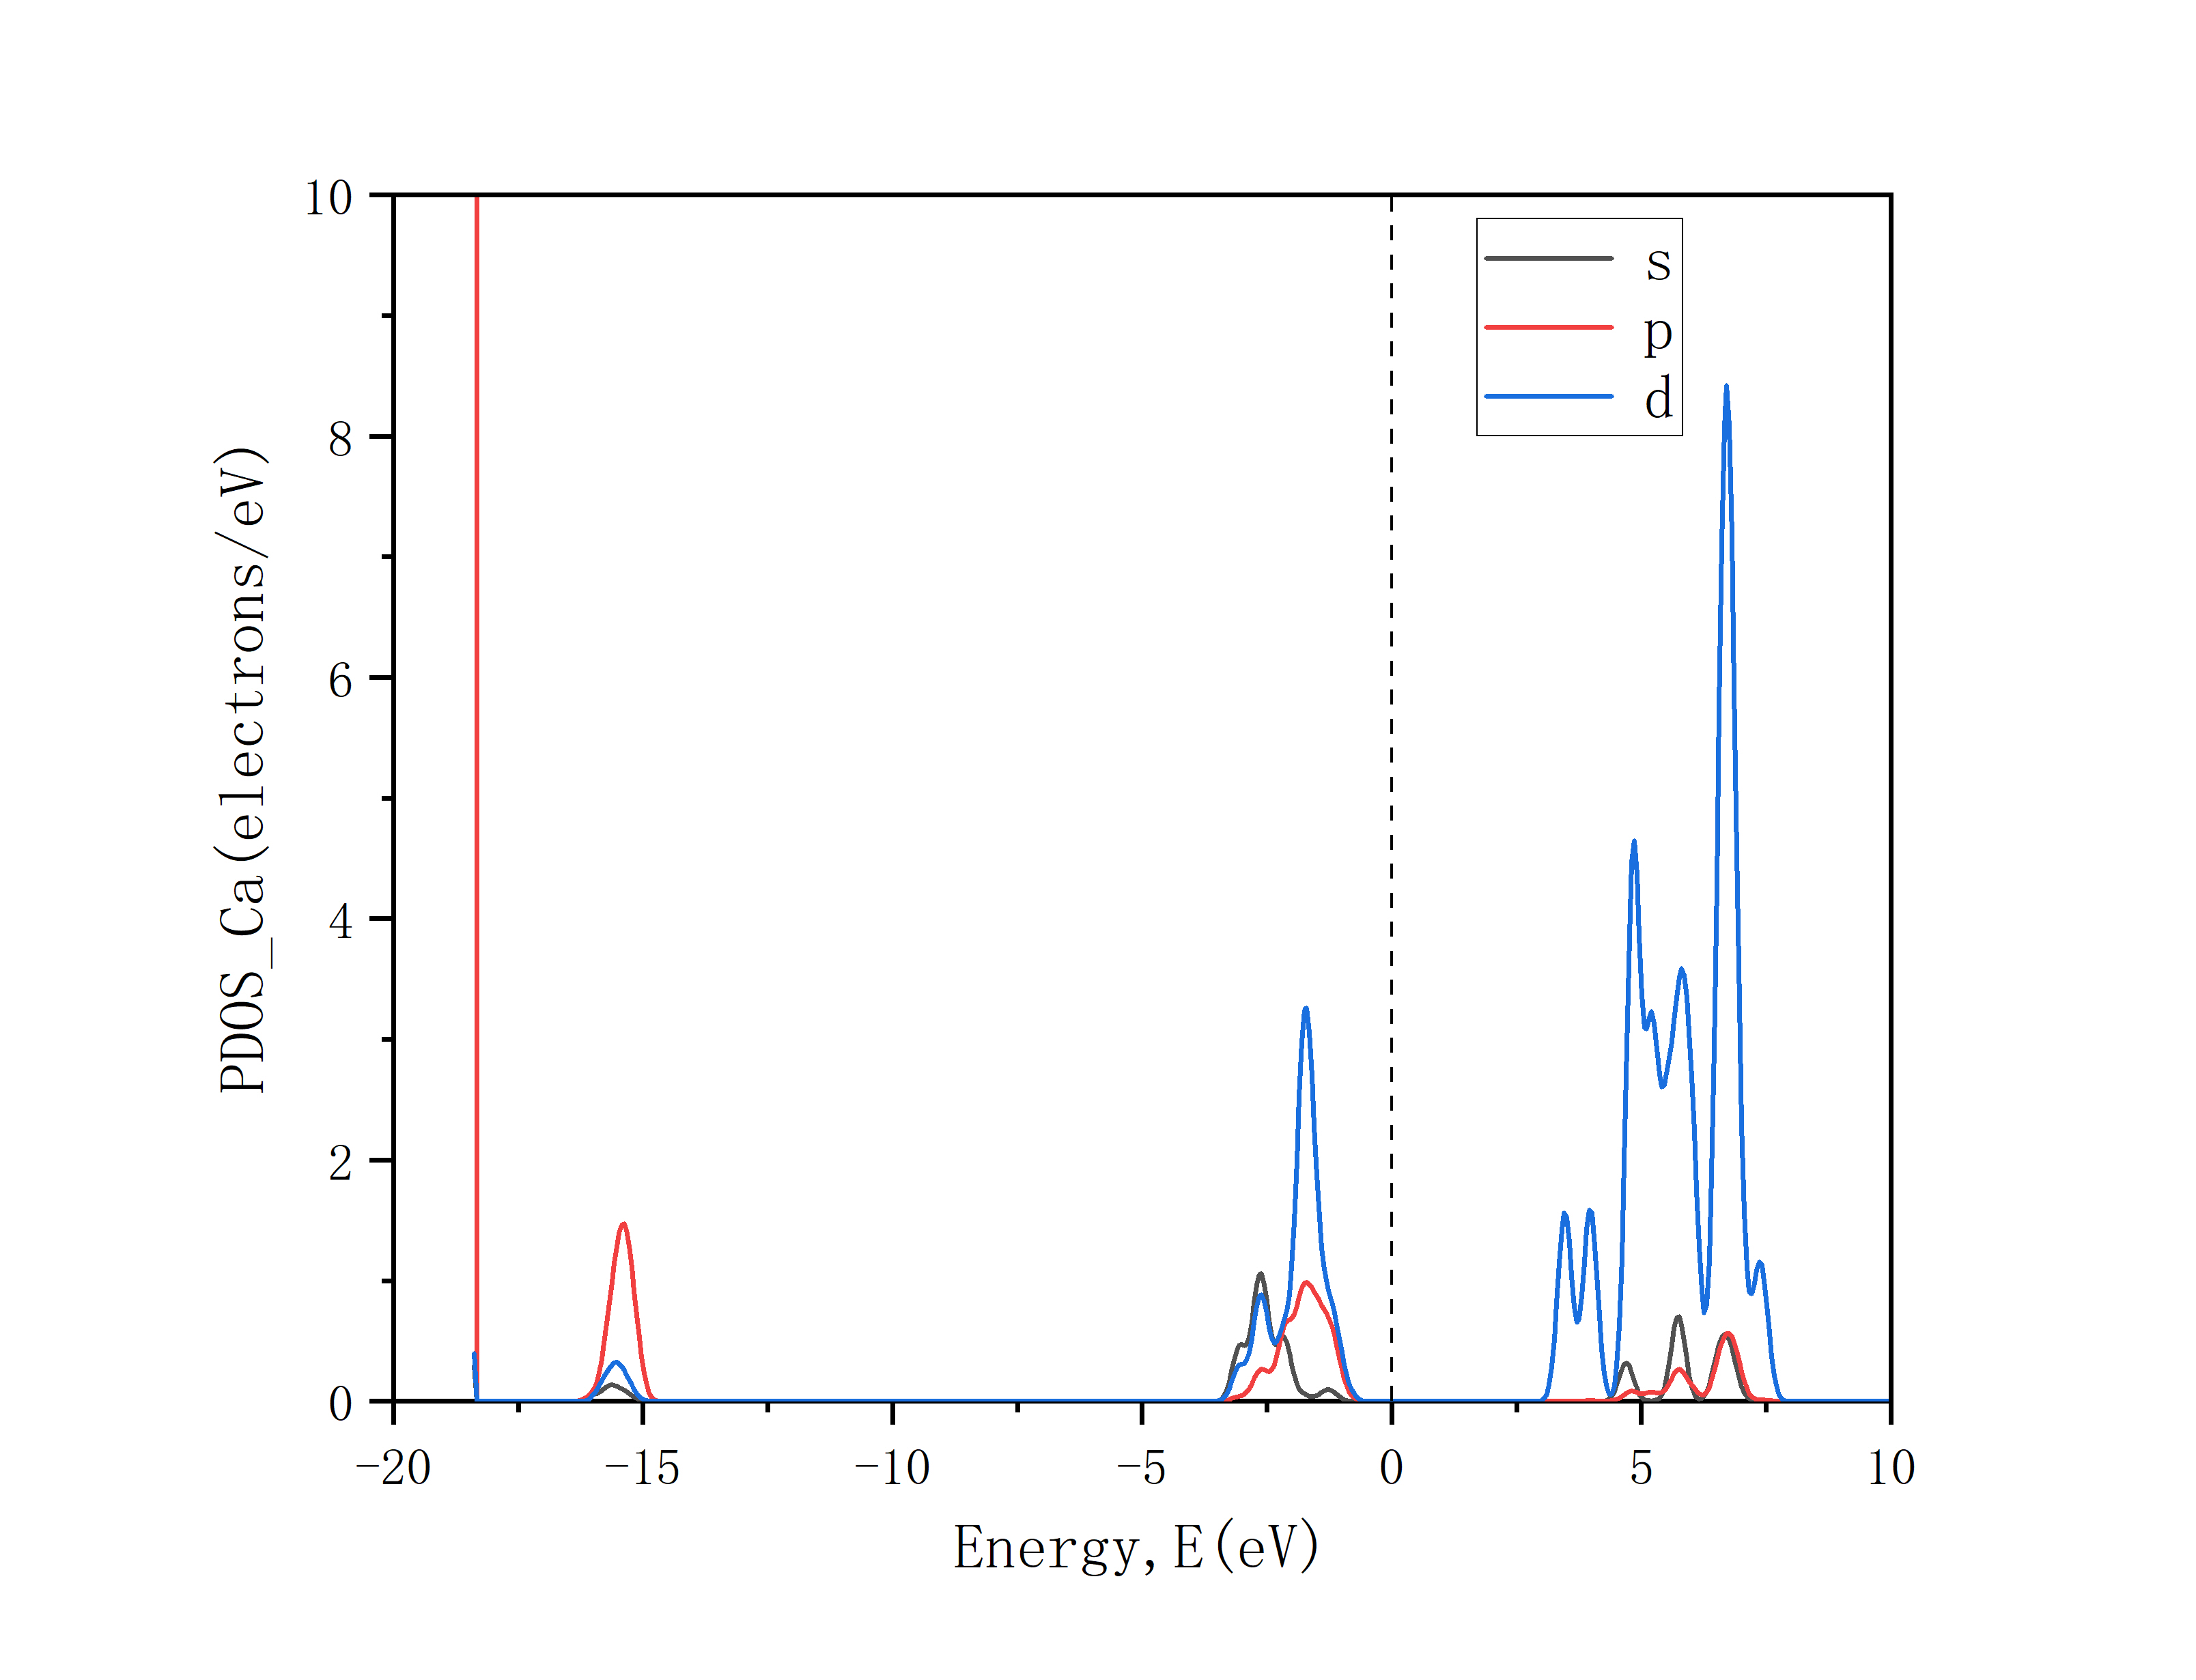
\includegraphics[width=0.45\textwidth]{img/PDOS_Ca.jpg}}
			\subfigure[O的分波态密度图]{				% 图片2
			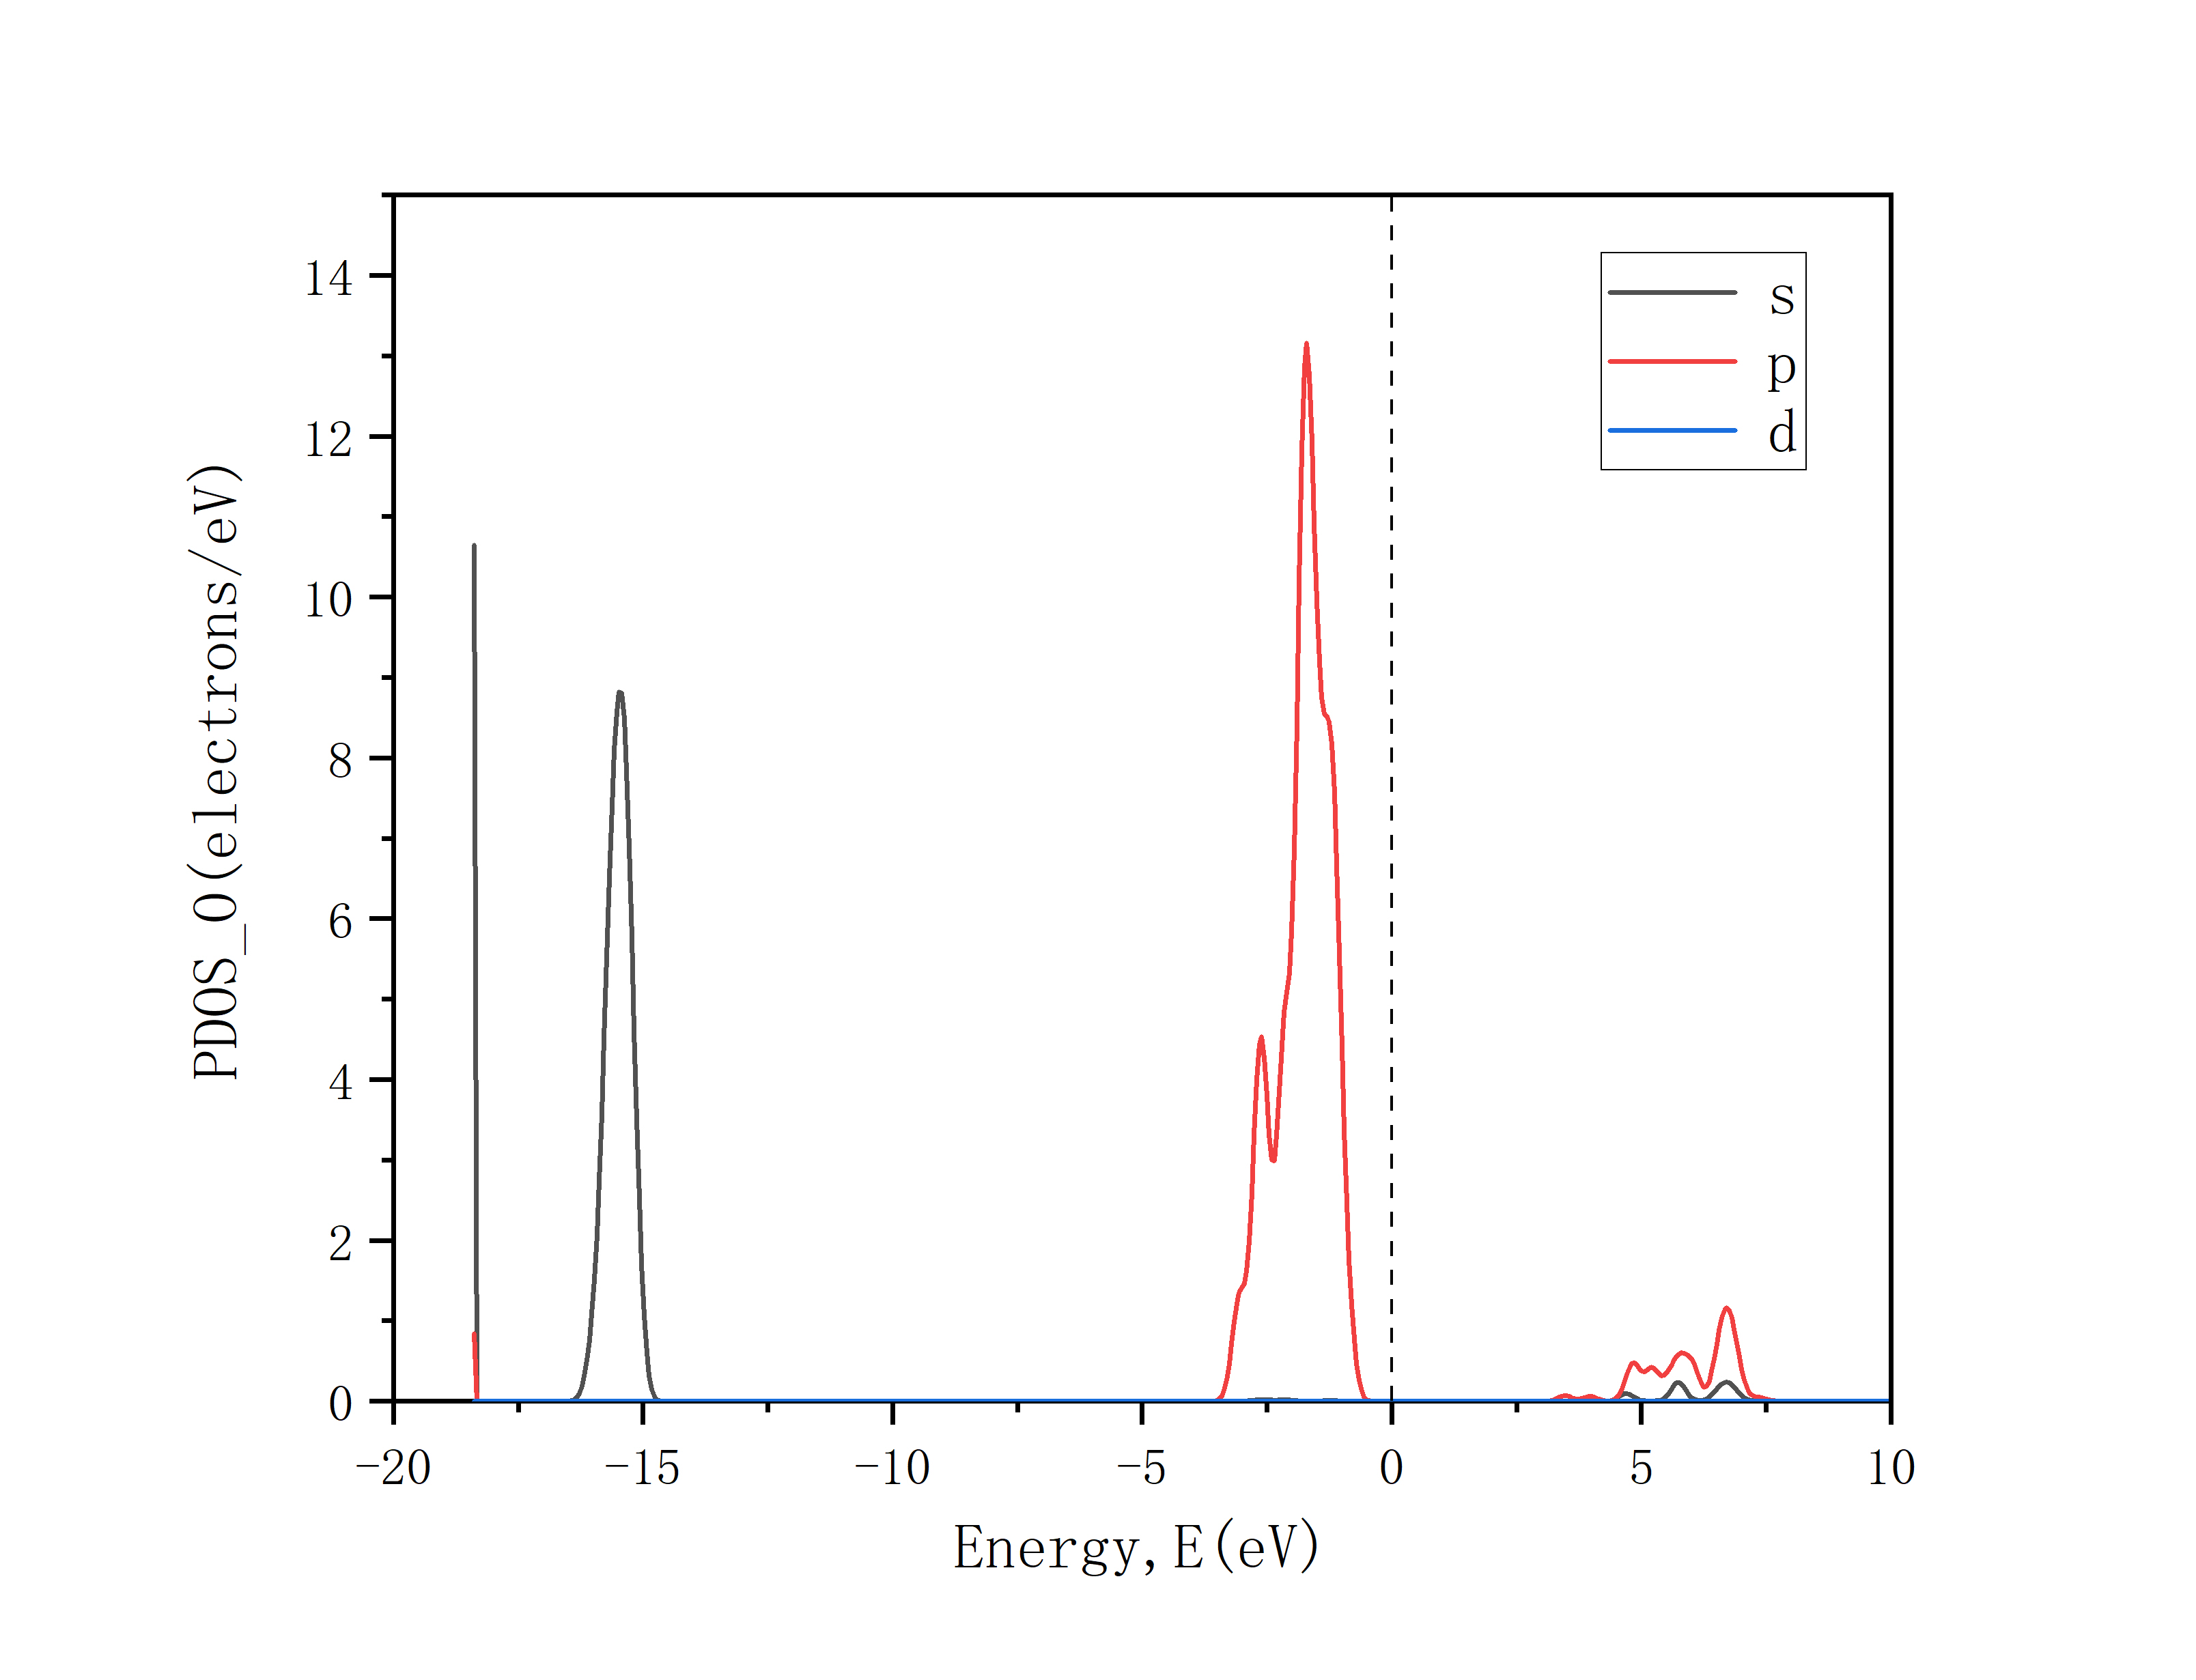
\includegraphics[width=0.45\textwidth]{img/PDOS_O.jpg}}
		\caption{CaO的态密度图} % 图片标题 
	\end{figure}
	为了深入理解CaO的成键特性,进一步计算了其电荷密度,并对其各个方向做出了对应的截面图3,其中中间原子带有红色的点的为O,没有带有红色点的为Ca。
	\begin{figure}[H]
		\centering    
		\subfigure[CaO晶胞体对角面截面]{				% 图片1([]内为子图标题)						
			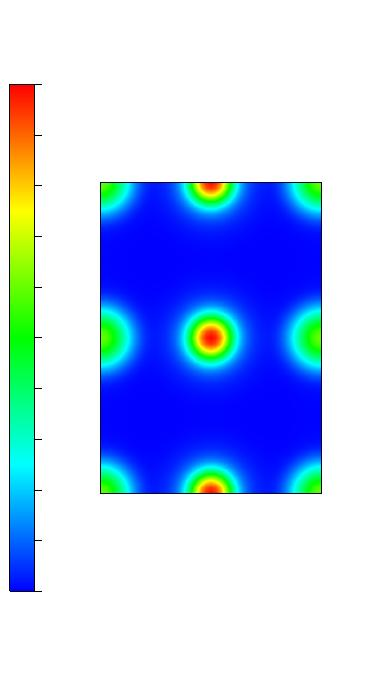
\includegraphics[width=0.43\textwidth]{img/CHGCAR.jpg}}			  % 子图1的图片宽度 不能空行
		\subfigure[CaO晶胞侧面截面]{				% 图片2
			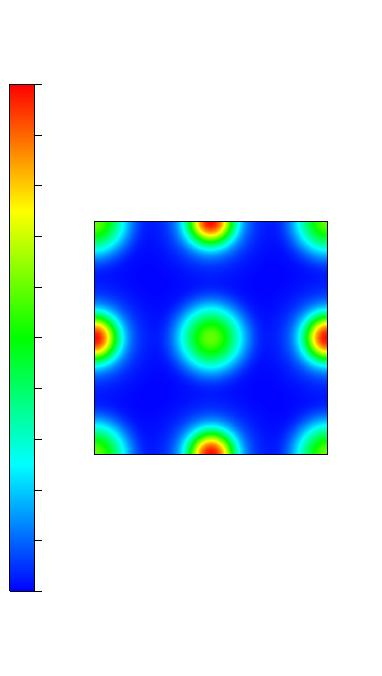
\includegraphics[width=0.45\textwidth]{img/CHGCAR侧视.jpg}}
		
		\caption{CaO的电荷密度分布} % 图片标题 
	\end{figure}
	从图3(a)和3(b)可以看到Ca原子的电子云与相邻的O原子之间发生强烈的杂化,且Ca与O之间的电子云重叠比Ca与Ca之间的强,表明Ca—O共价键强于Ca—Ca键。
		\subsection{能带结构}
	\vspace{-1cm}
	\begin{figure}[H]
		\centering
		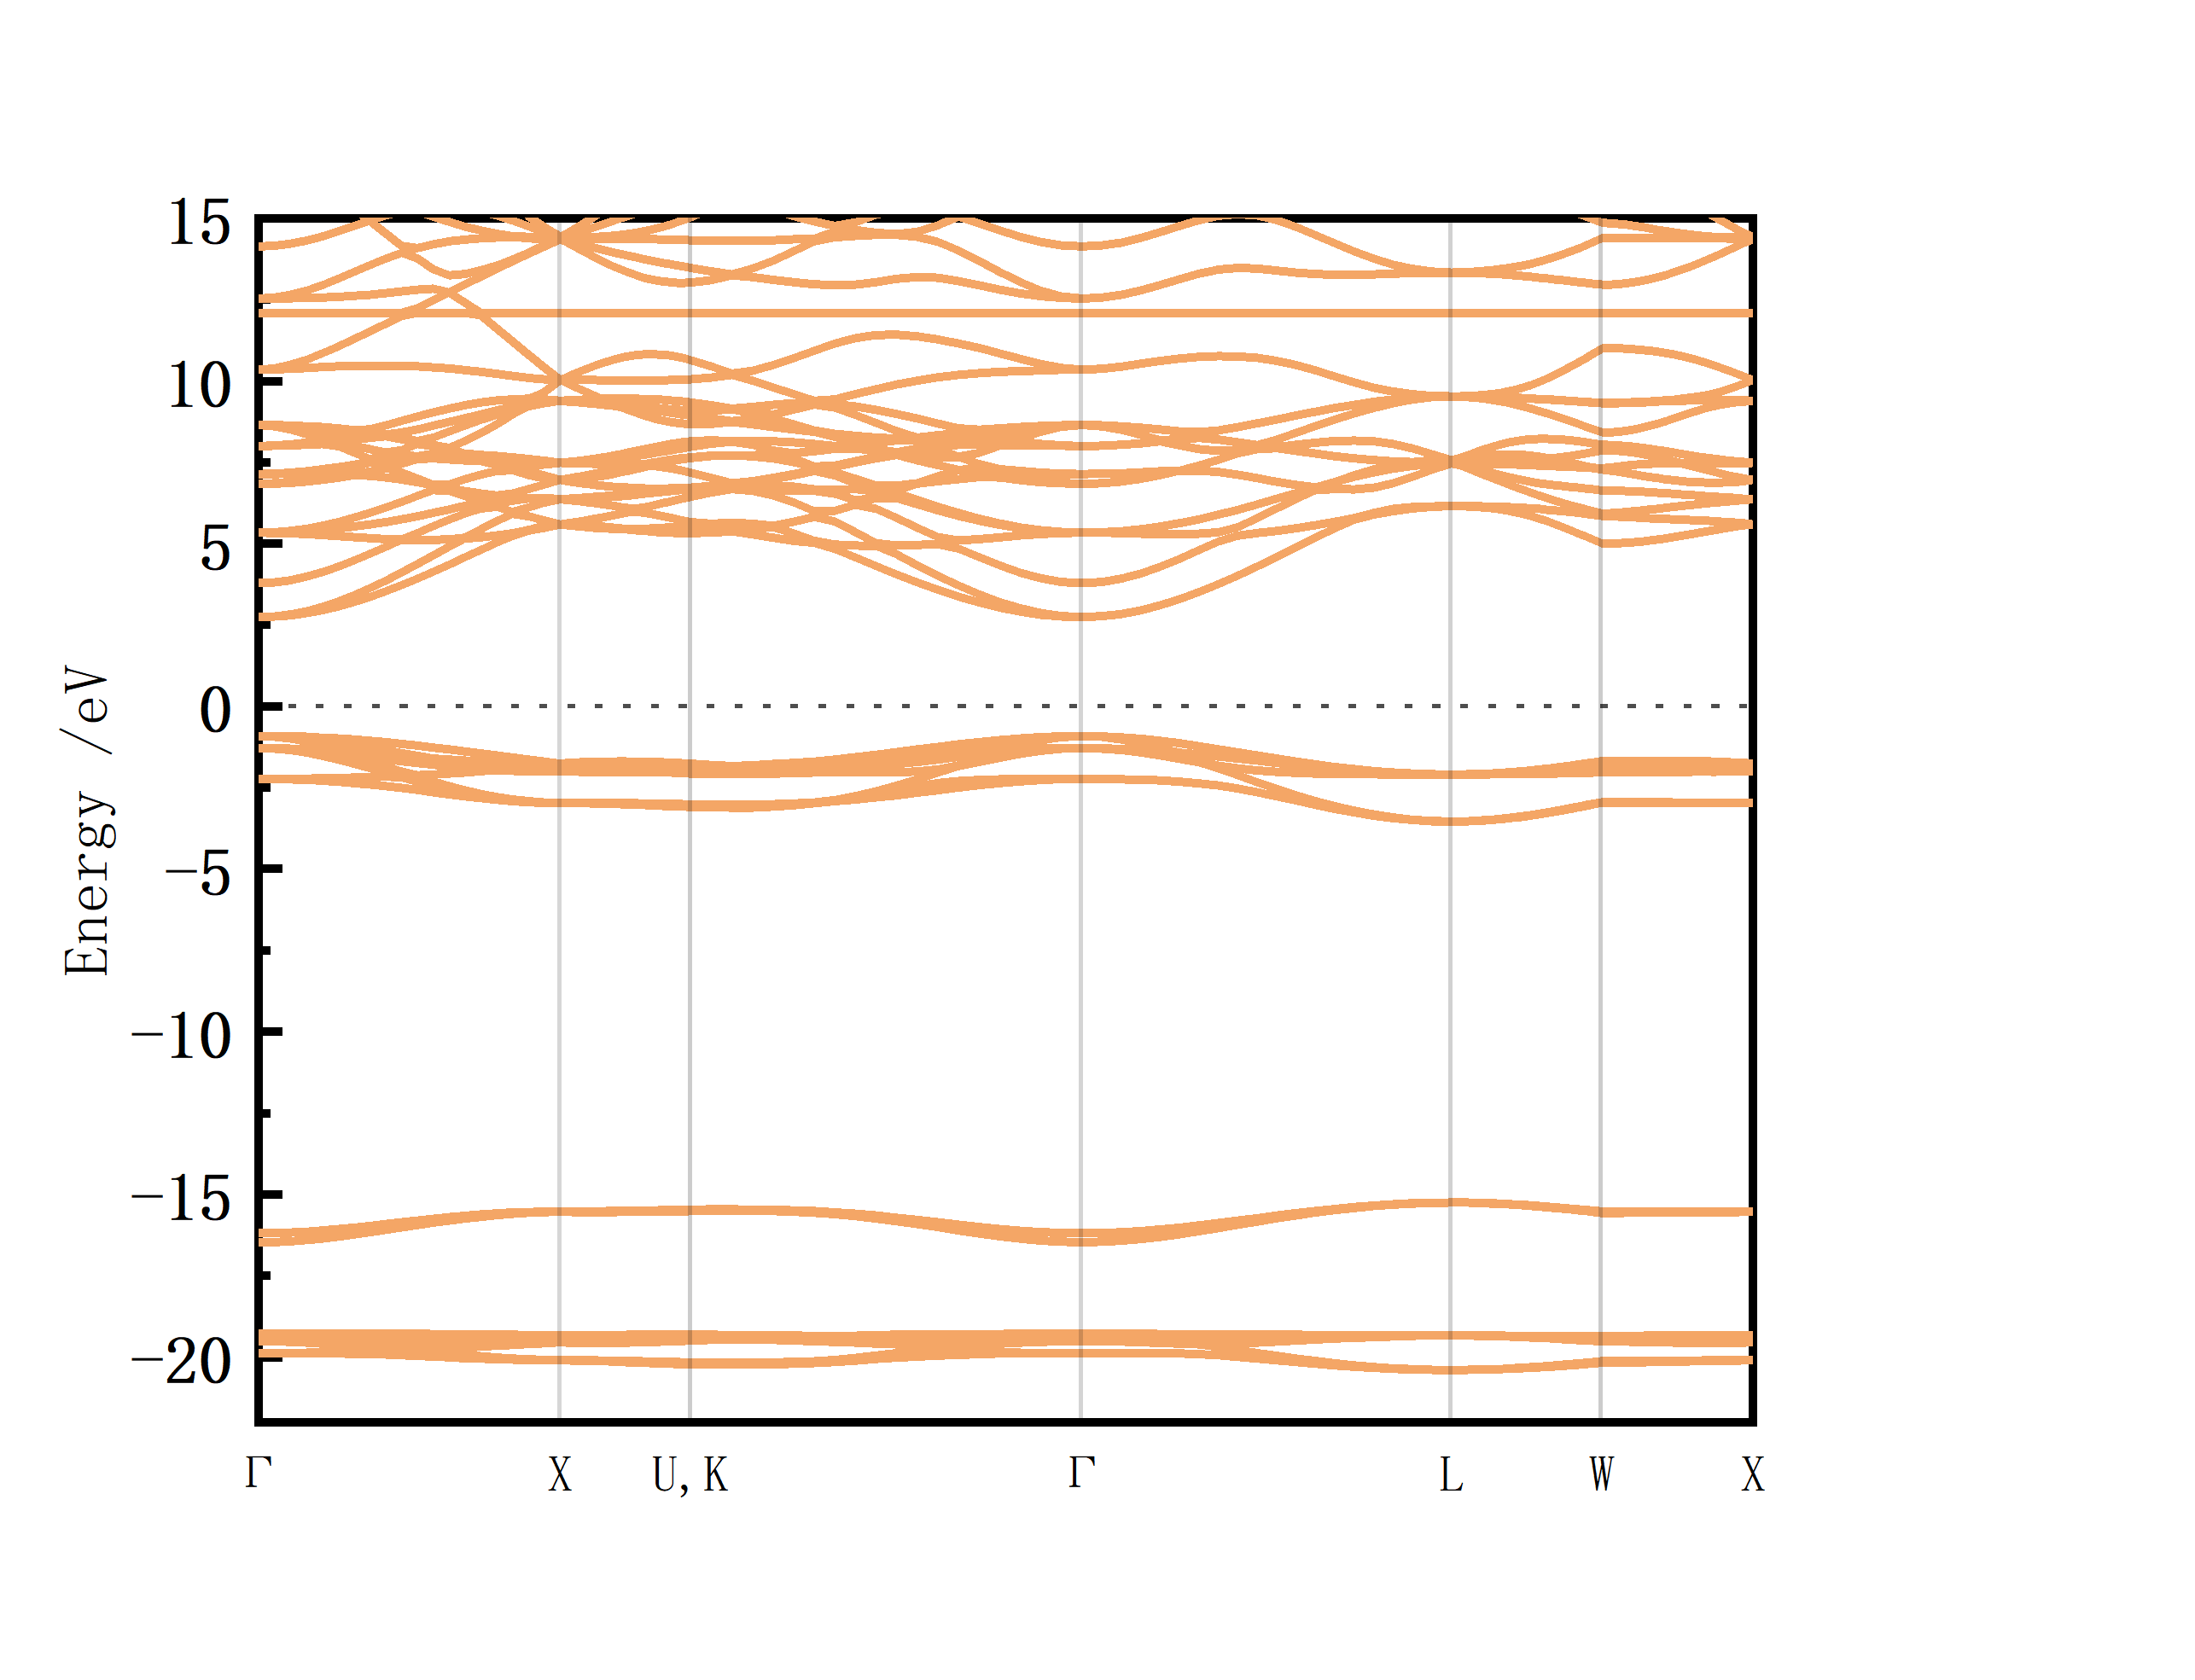
\includegraphics[width=0.55\linewidth]{img/能带图}
		\caption[CaO晶体的能带结构]{CaO晶体的能带结构}
		\label{fig:}
	\end{figure}
	\vspace{-0.8cm}
	图4是CaO的正交相的能带结构图,图中选取零点为费米能级。从图4可以看出,对于正交相的CaO结构,CaO的价带顶和导带底均位于
	$\Gamma$点,因此CaO是一种直接带隙绝缘体.计算得到CaO的带隙值为4.578 eV 。这与实验值7.1 eV$^{[11]}$存在一定
	差距,这种差异主要来源于GGA交换关联函数低估
	了体系激发态电子间的关联作用,但此差异并不影响
	对计算结果的定性分析。
	\section{结论}
	本研究采用基于密度泛函理论的第一性原理平
	面波赝势理论方法,对不同压强下CaO的能带结构、
	态密度进行理论计算与分析,结果表明:
	\begin{enumerate}
		\item 晶体优化后所得晶格常数与实验值较为吻
		合.经过对能带结构和态密度的分析表明CaO晶体属
		于直接带隙绝缘体,带隙值为4.578 eV,其价带顶和
		导带底分别由Ca—d轨道和O—p轨道贡献.
		\item CaO的成键特性中,由于Ca原子的电子云与相邻的O原子之间发生强烈的杂化,且Ca与O之间的电子云重叠比Ca与Ca之间的强,使得Ca—O共价键强于Ca—Ca键
	\end{enumerate}

	\newpage
	
	\begin{thebibliography}{99}% 参考文献,{}内表示序号最大位数(两位)
		\bibitem{1} DAI W, SHUI ZH, LI K, et al. First-principle investigations of CaO
		(100) surface and adsorption of H$_2$0 on CaO (100)[J]. Computational and Theoretical Chemistry, 2011, 967(1):185-190.
		\bibitem{2} GHEBOULI B, GHEBOULI M A, FATMI M, et al. First-principles calculations of structural, elastic, electronic and optical properties of $XO ( X= Ca , $ Sr and Ba$) $ compounds under pressure effect[J]. Materials Science in Semiconductor Processing, 2010, 13(2): 92-101.
		\bibitem{3} DUAN Y, QIN L, TANG C, et al. First-principles study of ground-and metastable-state properties of $XO(X=Be,Mg,Ca,Sr,Ba,Znand$ Cd)[J]. Eur Phys J B, 2008, 66(2): 201-209.
		\bibitem{4}  ANDREW J L, DAVID M F, DAVID O S, et al. Structural, energetio and electronic properties of (100) surfaces for alkaline earth metak oxides as calculated with hybrid density functional theory[J].Surface Science, 2015, 642: 58-65.
		\bibitem{5}  SU M X, YANG R, LI M. Biodiesel production from hempseed oil using alkaline earth metal oxides supporting copper oxide as bifunctional catalysts for transesterification and selective hydrogenation[J].Fuel, 2013, 103( 1 ): 398-407.
		\bibitem{6} WANG Z Y, LI X H, ZHANG Y, et al. Effect of alkaline-earth metal oxides on Cu/SiO$_2$-A$l_2$O$_3$ catalyst for vapor-phase synthesis of 3-methylindole from glycerol and aniline[J]. Chinese Journal of Catalysis, 2012, 33(7)$\colon$1139-1145.
		\bibitem{7} STAUDENRAUS J, EISENMENGER W. Fibre-optic probe hydrophone for ultrasonic and shock-wave measurements in water[J].Ultrasonics, 1993, 31(4): 267-273.
		\bibitem{8} LIJ, ZHOU X. A time-resolved single-pass technique for measuring optical absorption coefficients of window materials under 100 GPa shock pressure[J]. Review of Scientific Instruments, 2008,79(12); 123107.
		\bibitem{9}  RAVINDRAN P, DELIN A, AHUJA R, et al. Optical properties of monoclinic SnI$_2$ from relativistic first-principles theory[J]. Physical Review Ri Condensed Matter 1997,56(11),6851,6861
		\bibitem{10} http://condmatt.iphy.ac.cn/XRD/home
		\bibitem{11} 邢美静,梁凯,姚倩倩,等. 单轴应变下CaO和SrO电子结构和光学性质的第一性原理研究[J]. 天津师范大学学报(自然科学版),2016,36(3):21-27. DOI:10.3969/j.issn.1671-1114.2016.03.005.
		\bibitem{12} 刘峰斌,陈文彬,崔岩,等. 活性质吸附氢修饰金刚石表面的第一性原理研究?[J]. 物理学报,2016,65(23):236802-1-236802-9. DOI:10.7498/aps.65.236802.
		\bibitem{13} 李洺阳,吴苗苗,刘洋,等. CaO结构表面性质的第一性原理研究[C]. //中国矿业大学首届研究生教育发展论坛论文集. 2018:137-144.
		\bibitem{14} LOGSDAIL, ANDREW J., MORA-FONZ, DAVID, SCANLON, DAVID O., et al. Structural, energetic and electronic properties of (100) surfaces for alkaline earth metal oxides as calculated with hybrid density functional theory[J]. Surface Science: A Journal Devoted to the Physics and Chemistry of Interfaces,2015,642(Dec.):58-65. DOI:10.1016/j.susc.2015.06.012.
		\bibitem{15 } 刘亮,洪迪昆,冯于川,等. CaO基CO2吸附剂掺杂/负载活性组分的第一性原理[J]. 燃烧科学与技术,2017,23(5):412-417. DOI:10.11715/rskxjs.R201704006.
		\bibitem{16} 韦柳婷,童张法,吴东海,等. 氧化钙(100)、(110)和Ca-terminated(111)表面性能的第一性原理研究[J]. 广西科学,2015,22(6):670-674,680. DOI:10.3969/j.issn.1005-9164.2015.06.018.
	\end{thebibliography}
	
	
\end{document}% 结束文档编辑,后面写啥都编译不出来